110. Если провести высоту (и медиану) $BH,$ то $HC=AC:2=5,\ BH=\sqrt{169-25}=12.$ Тогда $S_{\Delta ABC}=\cfrac{1}{2}\cdot12\cdot10=60.$\\
а) Найдём площадь треугольника через проведённую из точки $C$ высоту $h:\ S=\cfrac{1}{2}h\cdot13=60,\ h=\cfrac{120}{13}.$\\
б) Найдём площадь треугольника через радиус вписанной окружности: $p=\cfrac{13+13+10}{2}=18,\ S=pr=18r=60,\ r=\cfrac{10}{3}.$\\
в) Найдём площадь треугольника через радиус описанной окружности: $S=\cfrac{abc}{4R}=\cfrac{13\cdot13\cdot10}{4R}=60,\ R=\cfrac{169}{24}.$\newpage\noindent
г) \begin{figure}[ht!]
\center{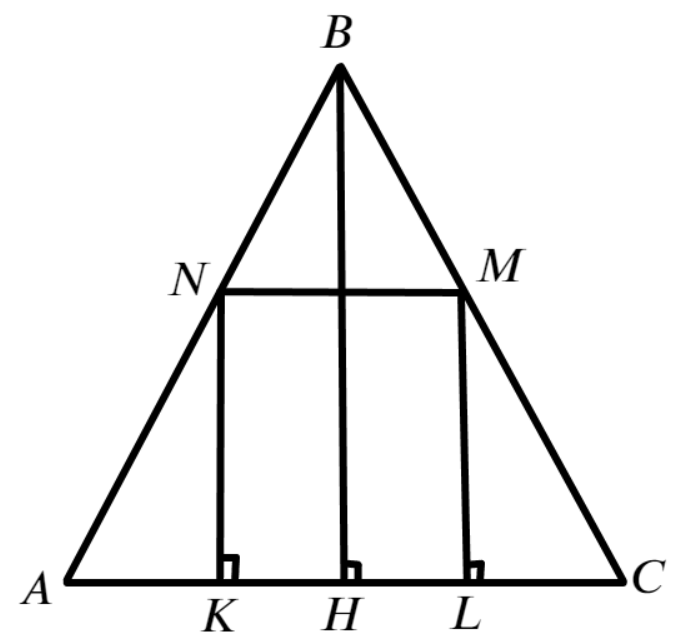
\includegraphics[scale=0.35]{g9-110.png}}
\end{figure}\\
Найдём $ctg(\angle A)=ctg(\angle C)=\cfrac{5}{12}.$ Тогда $AK=LC=LM\ ctg(\angle C)=\cfrac{5}{12}LM$ и $AC=2LC+KL=2\cdot\cfrac{5}{12}LM+\cfrac{1}{2}LM=\cfrac{4}{3}LM=10.$ Поэтому $KL=\cfrac{1}{2}LM=\cfrac{1}{2}\cdot\cfrac{15}{2}=\cfrac{15}{4}.$\\
